\documentclass[10pt]{book}
\usepackage{geometry}                % See geometry.pdf to learn the layout options. There are lots.
\usepackage{blindtext}
\usepackage[parfill]{parskip}    % Activate to begin paragraphs with an empty line rather than an indent
\usepackage{tikz}
\usetikzlibrary{arrows,automata,shadows,positioning,shapes}
\usepackage{graphicx}
\usepackage{amssymb}
\usepackage{amsmath}
\usepackage{amsthm}
\usepackage{epstopdf}
\usepackage{hyperref}
\usepackage{listings}
\usepackage{subfiles}
\usepackage[utf8]{inputenc}
\usepackage{float}
\usepackage{tikz}
\usepackage{graphicx}
\usepackage{caption}
\usepackage{wrapfig}
\usepackage{makecell}


\theoremstyle{definition}
\newtheorem{definition}{Definition}[section]


\title{High Performance Computing}

\begin{document}
\tableofcontents

%\input{01_Introduction/01_Introduction.tex}
\section{Modern Architectures}
    \subsection{Von Neuman architecture}
        \begin{enumerate}
            \item instruction decode: determine operation and operands
            \item fetch operands from memory
            \item perform some operations with them
            \item write the result back into memory
            \item continue with next instruction
        \end{enumerate}
        
        \begin{figure}
            \includegraphics{Von_Neuman_Architecture.png}
        \end{figure}
        
        
\chapter{Serial Optimization}
    There are two basic rules in optimization:
    \begin{enumerate}
        \item   In a world of highly parallel computer architectures only
                highly scalable codes will survive
        \item   Single core performance no longer matters since we have
                many of them and uses scalable codes
    \end{enumerate}
    But anyway, optimizing the serial code runtime also optimizes the
    parallel code runtime, since the code reduces the overall 
    amount of needed computer power. So \textbf{ the first goal when
    optimizing an existing code must be optimizing the serial code}.
    Figure \ref{SerOpt:SerOptAlg} 
    shows the steps how to optimize serial code.
    
    \begin{figure}[h]
        \centering
        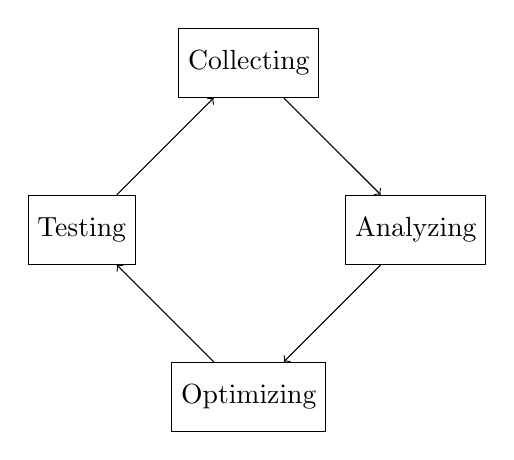
\begin{tikzpicture} [node distance = 3cm]
            \tikzstyle{every state}=[rectangle]
            \node[state]    (test)                              {Testing};
            \node[state]    (collect)   [above right of=test]   {Collecting};
            \node[state]    (analyze)   [below right of=collect]{Analyzing};
            \node[state]    (opt)       [below left of=analyze] {Optimizing};
            
            \path   (test)      edge[->]    (collect);
            \path   (collect)   edge[->]    (analyze);
            \path   (analyze)   edge[->]    (opt);
            \path   (opt)       edge[->]    (test); 
        \end{tikzpicture}
        \caption{Steps to improve serial code.}
        \label{SerOpt:SerOptAlg}
    \end{figure}
    
    Lets go a bit more into detail of the algorithem summed up in figure 
    \ref{SerOpt:SerOptAlg}. The first step must be collecting informations.
    There are serveral ways to get these informations,
    \begin{enumerate}
        \item   statically analysis of the source code
        \item   retrieving information about a programs runtime behavior
                (e.g. by \nameref{SerOpt:Profiling})
                $\rightarrow$ dynamic approach
        \item   Usually one determines how much time is spent in a certain
                function possibly identify \nameref{SerOpt:HotSpot}s
    \end{enumerate}
    If it is known where the most runtime is spent in, it is necessary to
    find out why so much time is spent in this part of the code. Therefore
    the collected data must because analyzed. The first step to the answer
    is to determine which factors stall the performance (e.g. by hardware
    counters). The next steps are obviously optimizing the code and testing.
    The size of the test is important. If the test size is to small the 
    performance behavior may not change signicantly. It if is to large the
    test may need to much time to be done. If testing is finished the 
    algorithm starts at data collection again.
    
    \begin{definition}[Hot Spot]    
        \label{SerOpt:HotSpot}
        Once there exists some kind of hotspot. In these
        hotspots $90\%$ of the runtime is spent, but the size of
        code, and so the size of the hotspot is only about $10\%$
        of the overall code. Nowadays this approximation does not hold in
        generals but hotspot analysis is still important.
    \end{definition}
    
    \section{Monitoring}
        \label{SerOpt:Monitoring}
        A common method for optimiziation a system's activities is 
        \emph{monitoring}. In the following there will be serveral definitions
        that are needed during the monitoring process.
        
        \begin{definition}[Event]
            \label{SerOpt:Event}
            An event is an predefined change in the systems's state. The
            definition depends on the measured metric, e.g. memory reference, 
            processor interrupts, appilaction processing, disk access, 
            network activity.
        \end{definition}
        
        \begin{definition}[Profile]
            \label{SerOpt:Profile}
            The profile is an aggregated picture of an application program. 
            For exampleaccumulated runtime spent in each function.
        \end{definition}
        
        \begin{definition}[Trace]
            \label{SerOpt:Trace}
            A trace is a log/sequenc of individual \nameref{SerOpt:Event}s.
            This includes event type and important system parameter.
        \end{definition}

        \begin{definition}[Overhead]
            \label{SerOpt:Overhead}
            The overhead is the Pertrubation introduced by the monitoring 
            technique.
        \end{definition}
        
        The level of the monitoring implementation can be devided up into
        \begin{enumerate}
            \item   Hardware monitoring
            \item   Software monitoring
            \item   Hybrid monitoring
        \end{enumerate}
        \subsection{Event- and sample driven triggers}
            For the monitoring there is some kind of trigger needed. One way
            is the \textbf{event-driven} triggers. With these triggers the
            performance measurement is done if and only if the pre-selected
            \nameref{SerOpt:Event} occurs. So the \nameref{SerOpt:Overhead}
            depend on the number of the pre-selected \nameref{SerOpt:Event}s.
            So the calculation of the \nameref{SerOpt:Overhead} is not easy.
            Furthermore this kind of trigger can significantly alter the 
            programs behavior. This trigger is good for tool with 
            low-frequency events. The other kind of trigger is called 
            \textbf{sample-driven} trigger. Here the performance is measured
            over snapshots at fixe time intervals. So the 
            \nameref{SerOpt:Overhead} of this technique is independent of the
            number of specific events. It takes snapshots on a specific
            frequency which the \nameref{SerOpt:Overhead} depends on. But 
            this trigger obviously does not have to measure every occurence of
            a specific \nameref{SerOpt:Event}, infrequent 
            \nameref{SerOpt:Event}s may not be covered at all. It just
            produces a statical view on the overall behavior of the system.
            So only very long runs are likely to produce a comparable result.
            view on the overall behavior of a system.
            
            \begin{table}[h]
                \centering
                \begin{tabular} {| l | l | l |}
                    & Event Trigger & Sample Trigger \\ \hline \hline
                    Precision & Exact & Probabilistic \\ \hline
                    Pertrubation & $O(f(N_{events}))$& fixed \\ \hline
                    overhead &  \makecell[l]{$O(f(N_{events}$)) \\ \\
                                Depends on: \\
                                    $\cdot$ event types instrumented \\
                                    $\cdot$ program behavior \\
                                    $\cdot$ overhead per event \\
                                } & 
                                \makecell[l]{ constant \\ \\
                                Depends on: \\
                                $\cdot$ Sampling rate \\
                                $\cdot$ Overhead per sample \\
                                }
                \end{tabular}
                \caption{Comparison between even- and sample-driven triggers.}
                \label{SerOpt:TriggerComp}
            \end{table}
        \subsubsection{Basic Block Counting}
            \label{SerOpt:BasicBlockCount}
            One way to implement monitoring is to use \textbf{Basic Block 
            Counting}. A \textbf{basic block} is a sequence of instructions that
            has no branches in or out of the sequence. This method just adds an
            instruction to the block to count the number of times the block is
            executed. After the termination the measurements from an execution
            can be represented as an histogram. In contrary to sample-driven
            trigger, block counting gives the exact number of times a block was
            executed. But this method also includes a siginficant runtime 
            overhead. This is the reason why block counting can have a severe
            impact on program's behavior/performance.
        
        \subsubsection{Instrumentation}
            \label{SerOpt:Instrumentation}
            This is another option to implement an event-driven trigger.
            Therefore additional instructions are put into the program for
            monitoring certain components (usually at least runtime).
            The instrumented code triggers the event during the runtime.
            An event could be entering or exiting a certain function/
            basic block. This method is allready implemented. This
            is a list of possible implementations:
            \begin{enumerate}
                \item Source code modifications (manual instructions)
                \item software exceptions
                \item emulation
                \item library
                \item modification by the compiler
            \end{enumerate}
            The advantage of \nameref{SerOpt:Monitoring} with manual instructions 
            is that the programmer can choose which part of the program is worth
            measuring and which is not. So possible \nameref{SerOpt:HotSpot}s
            can be preselected.
            The disadvantage is, that these \nameref{SerOpt:Monitoring} is not
            automic which means that it is time consuming. Furthermore it is
            error prone and non-experienced programmers may think that they 
            have a clear understand of the program's workflow and miss 
            non-obvious \nameref{SerOpt:HotSpot}s. \\
            For \nameref{SerOpt:Monitoring} with software exceptions a specific
            tpye of precessor is need. Not all processors support software
            exceptions just before the execution on each instruction. The
            exception handler can be installed to interpret the instruction and
            its operands.
            The advantages are that this way of \nameref{SerOpt:Monitoring} 
            is very detailed and accurate but in general it is far too detailed
            and too low-level to enable an easy interpretation of the workflow. \\
            \nameref{SerOpt:Monitoring} with the help of emulation means that
            an emulator makes the system it is running on look like something
            completely different to the outside. The Java Virtual Machine is
            such and emulator. It interprets the Java byte-code, translates it
            into machine instructions and emulates a processor that can 
            interpret java byte-code. instruction format. For emulation 
            \nameref{SerOpt:Tracing} can easily be implemented but the
            emulation is slow compared to native code execution. \\
            For \nameref{SerOpt:Monitoring} while runtime there are also 
            libraries given. One if them is for example OpenMP. These libraries
            can either be instrumented or covered by instrumentation-wrapper
            replacements. This gives quite a good overview on the program's
            behavior. \\
            Finaly modifications can be done by the compiler. The compiler can
            add instrumentation instructions to the executable code it compiled
            automatically. Similar to basic block profiling. There are two ways
            to use this compiler modifications. Either a compilation option is
            used or a post-compilation software tool is used. The advantage is
            that everything is fully automatic. The overhead depends on how
            often functions are called and usually different compiler options
            can control the overhead.
            


\end{document}

